\chapter{Introduction}
\label{chap:introduction}
\section{Motivation} 
\label{sec:motivation}
In the domain of computational finance, much research is performed to find and improve algorithms that help maximize revenue. One possibility to maximize revenue is to minimize inevitably occurring costs: In the first place, investors participating in exchange markets, must expect fees, charged by the respective market place organizer in return for granting access to their infrastructure. On the other hand, there are hidden costs to be considered as well.\\

In most exchange markets, the actual price of an asset is controlled by supply and demand, where a universe of opposing trading interests determines the \emph{fair} price of a commodity. While trades involving little capital\footnote{Little capital, relative to the whole market liquidity.} usually cause minor impact on the current market situation, large-scale investors must be cautious when it comes to order placements. Large orders can have a major impact on supply and demand, leading to diminishing availability and worsening prices, that must be seen as \emph{hidden costs}.\\

While direct costs are contractually regulated and thus predictable to a large extend, this is not the case for hidden costs. The unpredictable nature of hidden costs bears a significant risk that grows exponentially with the trading volume pursued. This motivates for well considered trading strategies, that help to reduce the investors impact and avoid costly market turbulences by unwinding large orders of shares over time. \\



\section{Objectives}
\label{sec:objectives}
This thesis tackles the important problem of \emph{optimized trade execution}, which frequently occurs in the domain of financial computing. In its simplest form, the problem is defined by a particular financial instrument (here: bitcoins), which must be bought or sold within a fixed time horizon, while minimizing the expenditure (share price) for doing so.\\

\begin{figure}[ht]
	\centering
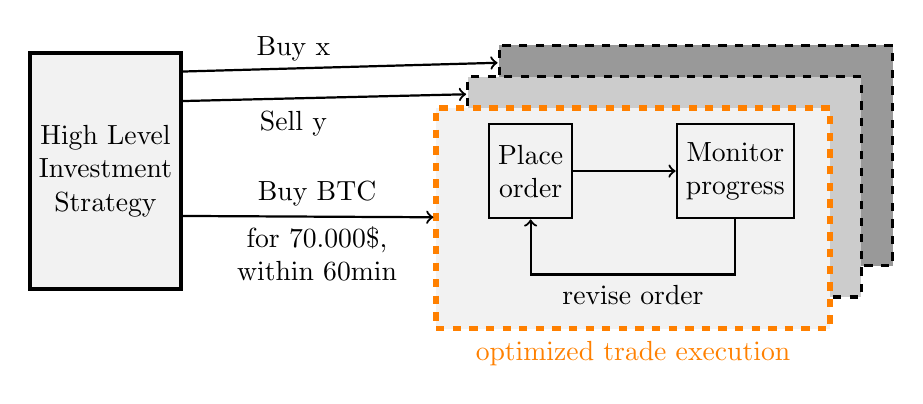
\begin{tikzpicture}[node distance = 16em, auto, thick]
    \node[draw, minimum height=3cm, align=center, fill=black!5, line width=0.5mm] at (0, 0)   (A) {High Level\\Investment\\Strategy};
    \node[draw, black, dashed, minimum height=2.8cm, minimum width=5cm, line width=0.4mm, fill=black!40] at (7.5,0.2) (X2) {};
    \draw[->] (A.52) node[above, xshift=2.7cm] {}  node[above, align=center, xshift=1.4cm]{Buy x}  -- (X2.155);
    
    \node[draw, black, dashed, minimum height=2.8cm, minimum width=5cm, line width=0.4mm, fill=black!20] at (7.1,-0.2) (X1) {};
    \draw[->] (A.42) node[above, xshift=2.7cm] {}  node[below, align=center, xshift=1.4cm]{Sell y} -- (X1.155);

    \node[draw, orange, dashed, minimum height=2.8cm, minimum width=5cm, line width=0.7mm, fill=black!5, label={below, orange: optimized trade execution}] at (6.7,-0.6) (X) {}; 
%    \draw[->] (A) node[above, xshift=2.7cm] {}  node[below, align=center, xshift=2.7cm]{Sell x} -- (X1);

%    \node[draw, minimum height=2.8cm,minimum width=5cm, label={below: optimized trade execution}] {xx} ;


    

    \node[draw, minimum height=1.2cm, align=center] at (5.4, 0)   (B) {Place\\order};
    \node[draw, minimum height=1.2cm, align=center] at (8, 0)   (C) {Monitor\\progress};
%    \node[draw, minimum height=1.2cm, align=center] at (11, 0)   (D) {done};
%    \node[draw] at (12, 0)   (E) {Application};

    
    \draw[->] (A.-30) node[above, xshift=1.7cm] {Buy BTC}  node[below, align=center, xshift=1.7cm]{for $70.000\$$,\\within 60min} -- (X);

    \draw[->] (C.south) node[below, xshift=-1.3cm, yshift=-0.7cm] {revise order}  -- ++(-0,0) -- ++(0,-0.7) -| (B);

    \draw[->] (B) node[above, xshift=2.1cm] {}  -- (C);

%    \draw[->] (C) node[above, xshift=2.1cm] {}  -- (D);

\end{tikzpicture}
	\caption{Scope of this thesis.}
	\label{fig:objectives}
\end{figure}

The scope of this thesis is to transfer Nevmyvakas \cite{Nevmyvaka:2006} reinforcement learning approach from traditional stock markets with expensive, proprietary data sources, to the relatively young market of bitcoin trading and to improve it's general ability to solve the important problem of optimized trade execution. In contrast to their experiments this thesis builds on inexpensive, publicly retrievable bitcoin exchange data. Snapshots of the current market situation are retrieved on a low-resolution, minute-scale basis from the open bitcoin exchange platform Poloniex. As such the usability of the retrieved dataset remains to be shown. \\

Additional market features, describing the current market situation as well as historic market performance, are evaluated in terms of cost impact. An Orderbook Trading Simulator (OTS), which simulates the individual traders influence on the current market situation, is implemented and used in order to learn and evaluate various trading strategies.


\section{Related Work}
\label{sec:relatedwork}
x

\section{Contributions}
\label{sec:contributions}
\begin{itemize}
\item An orderbook trading simulator framework is presented which takes into account the individual traders influence on the current market situation.

\end{itemize}

\section{Outline of Contents}
\label{sec:outline}
The remainder of this thesis is structured as follows:\\
\Cref{chap:background} gives a general introduction into the vocabulary of financial computing and the machine learning techniques employed, \Cref{chap:simulator} describes the Orderbook Trading  Simulator, developed within the scope of this thesis, and \Cref{chap:reinforcementlearning} covers the machine learning part. \Cref{chap:conclusion} closes with a conclusion and discussion.


\cleardoublepage{}